\documentclass[11pt]{article}
\usepackage{graphicx}
\usepackage{siunitx}
\usepackage{cleveref}
\usepackage{keyval,kvoptions,fancyvrb,float,ifthen,calc,ifplatform,pdftexcmds,etoolbox,lineno}
\usepackage[utf8]{inputenc}
\usepackage[danish]{babel}
\usepackage[left=25mm, right=25mm, top=25mm, bottom=25mm]{geometry}
\usepackage{amsthm}
\setlength\parindent{0pt}
\usepackage{dcolumn}
\usepackage{minted}
\usepackage{setspace}
\usepackage{tabularx}

\title{Dokumentation}

\begin{document}

\begin{titlepage}

\newcommand{\HRule}{\rule{\linewidth}{0.5mm}} % Defines a new command for the horizontal lines, change thickness here

\center % Center everything on the page
 
%----------------------------------------------------------------------------------
%	HEADING SECTIONS
%----------------------------------------------------------------------------------

\textsc{\LARGE Aarhus School of Engineering}\\[1.0cm] % Name of your university/college
\textsc{\Large 2.SEMESTERPROJEKT}\\[0.1cm]
\textsc{\large E2PRJ2}\\[0.3cm]
\textsc{\large gruppe 10}\\[0.3cm] % Minor heading such as course title

%----------------------------------------------------------------------------------
%	TITLE SECTION
%----------------------------------------------------------------------------------

\HRule \\[0.4cm]
{ \huge \bfseries Smart Morning System - SMS}\\[0.1cm] % Title of your document
\HRule \\[0.6cm]

%----------------------------------------------------------------------------------
%	DATE SECTION
%----------------------------------------------------------------------------------

{\large \today}\\[0.5cm] % Date, change the \today to a set date if you want to be precise
 
%----------------------------------------------------------------------------------
%	AUTHOR SECTION
%----------------------------------------------------------------------------------

\begin{minipage}[t]{0.4\textwidth}
\raggedright \large
\emph{Forfattere:}\\
\begin{tabular}[t]{@{}r@{ }l@{}}
	201511621 & \textbf{Christian Brandstrup Bondesen}\\
	201511621 & \textbf{Emil Celik}\\
	201408914 & \textbf{Marc Auphong Bui}\\
	2015xxxxx & \textbf{Rasmus Lund}\\
	201406253 & \textbf{Simon Egeberg}\\
  \end{tabular}
\end{minipage}
~
\begin{minipage}[t]{0.4\textwidth}
\raggedleft \large
\emph{Vejleder:} \\
\textbf{Kim Bjerge} % Supervisor's Name
\vfill
\end{minipage}\\[0.8cm]


%----------------------------------------------------------------------------------
%	LOGO SECTION
%----------------------------------------------------------------------------------
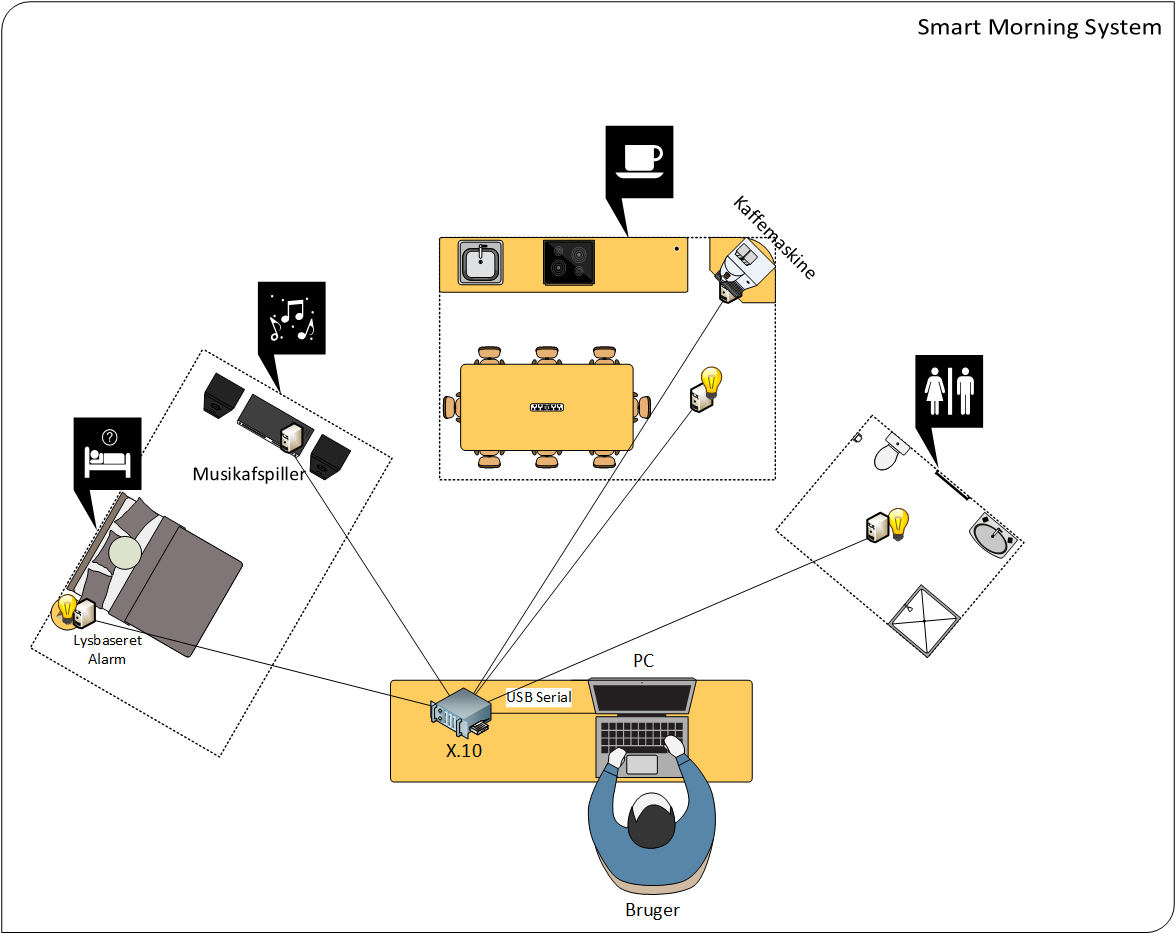
\includegraphics[scale=0.6]{projektillustration.png}\\[0.6cm]

\includegraphics[scale=0.25]{forsidelogo.jpg}\\[1cm] % Include a department/university logo - this will require the graphicx package
%----------------------------------------------------------------------------------
\vfill % Fill the rest of the page with whitespace

\end{titlepage}

\tableofcontents
\vfill
\pagebreak

\section{Indledning}
\vfill
\pagebreak

\section{Kravspecifikation}
%Tabeloversigt over hovedansvarsområder for projektdeltagerne
\vfill
\pagebreak

\section{Arkitektur}
\vfill
\pagebreak

\section{Hardware-design, implementering \& modultest}
\subsection{Design (HW)}
\subsection{Implementering (HW)}
\subsection{Modultest (HW)}
\vfill
\pagebreak

\section{Software-design, implementering \& modultest}
\subsection{Design (SW)}
\subsection{Implementering (SW)}
\subsection{Modultest (SW)}
\vfill
\pagebreak

\section{Integrationstest (HW/SW)}
%Valgfrit på 2.semester
\vfill
\pagebreak

\section{Accepttest}
\vfill
\pagebreak

\section{Bilag}
\vfill
\pagebreak



\end{document}